% Fig. 1 of main.tex. Compile: pdflatex fig_pipeline
\documentclass[border=1pt]{standalone}
\usepackage{amsmath,amssymb}
\usepackage{tikz}
\usetikzlibrary{positioning,arrows.meta,fit,calc}
\begin{document}
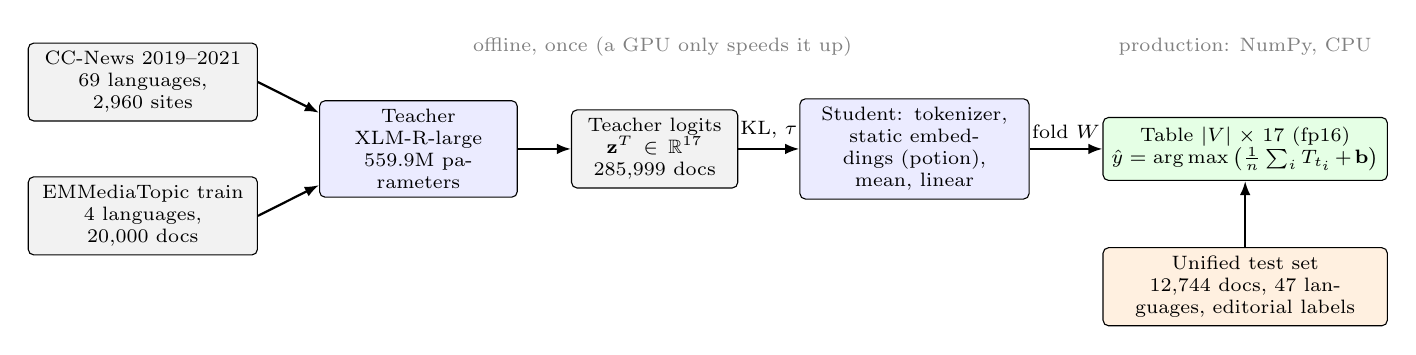
\begin{tikzpicture}[
  box/.style={draw, rounded corners=2pt, align=center, font=\scriptsize, inner sep=3pt, minimum height=8mm},
  data/.style={box, fill=gray!10},
  model/.style={box, fill=blue!8},
  prod/.style={box, fill=green!10},
  test/.style={box, fill=orange!12},
  arr/.style={-{Latex[length=1.8mm]}, thick},
  lab/.style={font=\scriptsize}]
  \node[data, text width=27mm] (cc)  at (1.4, 0.85)  {CC-News 2019--2021\\69 languages, 2,960 sites};
  \node[data, text width=27mm] (emm) at (1.4,-0.85)  {EMMediaTopic train\\4 languages, 20,000 docs};
  \node[model, text width=23mm] (t)  at (4.9, 0)     {Teacher\\XLM-R-large\\559.9M parameters};
  \node[data, text width=19mm] (soft) at (7.9, 0)    {Teacher logits\\$\mathbf{z}^{T}\in\mathbb{R}^{17}$\\285,999 docs};
  \node[model, text width=27mm] (s)  at (11.2, 0)    {Student: tokenizer,\\static embeddings (potion),\\mean, linear};
  \node[prod, text width=34mm] (tab) at (15.4, 0)    {Table $|V|\times 17$ (fp16)\\$\hat{y}=\arg\max\big(\frac{1}{n}\sum_i T_{t_i}+\mathbf{b}\big)$};
  \node[test, text width=34mm] (ts) at (15.4, -1.75)  {Unified test set\\12,744 docs, 47 languages, editorial labels};
  \draw[arr] (cc.east)  -- (t.160);
  \draw[arr] (emm.east) -- (t.200);
  \draw[arr] (t) -- (soft);
  \draw[arr] (soft) -- node[lab, above]{KL, $\tau$} (s);
  \draw[arr] (s) -- node[lab, above]{fold $W$} (tab);
  \draw[arr] (ts.north) -- (tab.south);
  \node[lab, text=gray] at (8.0, 1.3) {offline, once (a GPU only speeds it up)};
  \node[lab, text=gray] at (15.4, 1.3) {production: NumPy, CPU};
\end{tikzpicture}
\end{document}
